%*----------- SLIDE -------------------------------------------------------------
%*----------- SLIDE -------------------------------------------------------------
\begin{frame}[c]{\textit{Monte Carlo localization}}
    \begin{center}
    
        \includemedia[
            width=0.7\linewidth,
            totalheight=0.39375\linewidth,
            activate=pageopen,
            passcontext, 
            %transparent,
            addresource=./Source/movies/Montecarlo_localization.mp4,
            flashvars={
            source=./Source/movies/Montecarlo_localization.mp4
            &autoPlay=true
            &autoRewind=true
            &loop=true}
            ]
            {\fbox{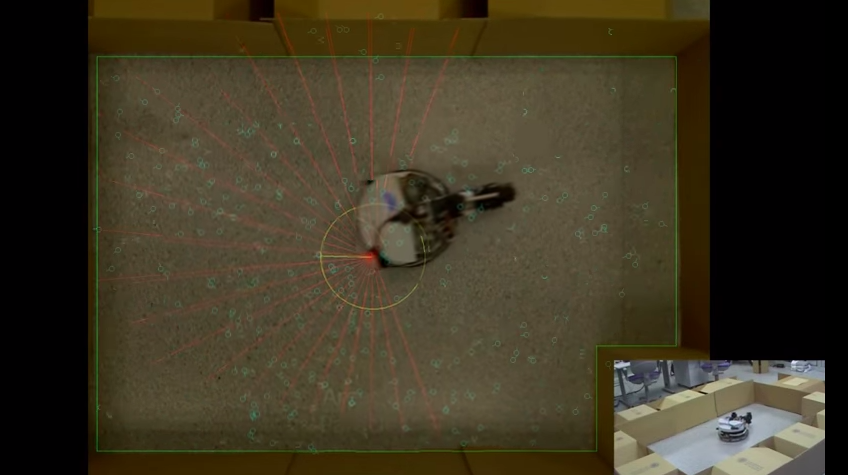
\includegraphics{Source/movies/montecarlo.png}}}{VPlayer.swf}
            
            Monte Carlo localization\cite{Montec41:online}
    \end{center}

 \end{frame}
%*----------- SLIDE -------------------------------------------------------------
\begin{frame}[c]{\textit{Monte Carlo localization}}
    Para obter a posição do robô é mantido:

    \begin{itemize}
        \item uma densidade de probabilidade da localização do robô dentro de determinado tempo;
        \item todas as observações por tempo;
        \item todas as entradas de controle por tempo.
    \end{itemize}

\end{frame}

%*----------- SLIDE -------------------------------------------------------------
\begin{frame}[c]{\textit{Monte Carlo localization}}
    E para atualizar os dados da posição são alternados dois estados
    \newline

    \begin{center}
        \begin{figure}
            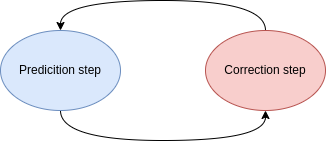
\includegraphics[width=0.5\textwidth]{Untitled Diagram.drawio.png}
        \end{figure}
    \end{center}

\end{frame}


%*----------- SLIDE -------------------------------------------------------------
\begin{frame}[c]{\textit{Prediction Models for MLS maps}}
    O \textit{prediction model} é feito da seguinte forma:

    % \begin{columns}[t]
    %     \column{.05\linewidth}
    %     \column{.5\linewidth}
    %         \begin{enumerate}
    %             \item obtêm um possível resultado para a ação aplicando um modelo probabilístico;
    %             \item adapta o vetor de movimento com base nos pedaços de superfície obtidos no MLS map;
    %             \item conseguimos a posição e orientação;
    %             \item com exceção do parâmetro de altura (z)  que tem que ser ajustado manualmente.
    %         \end{enumerate}
    %     \column{.6\linewidth}
        \begin{center}
        %\centerline{
            \begin{figure}
                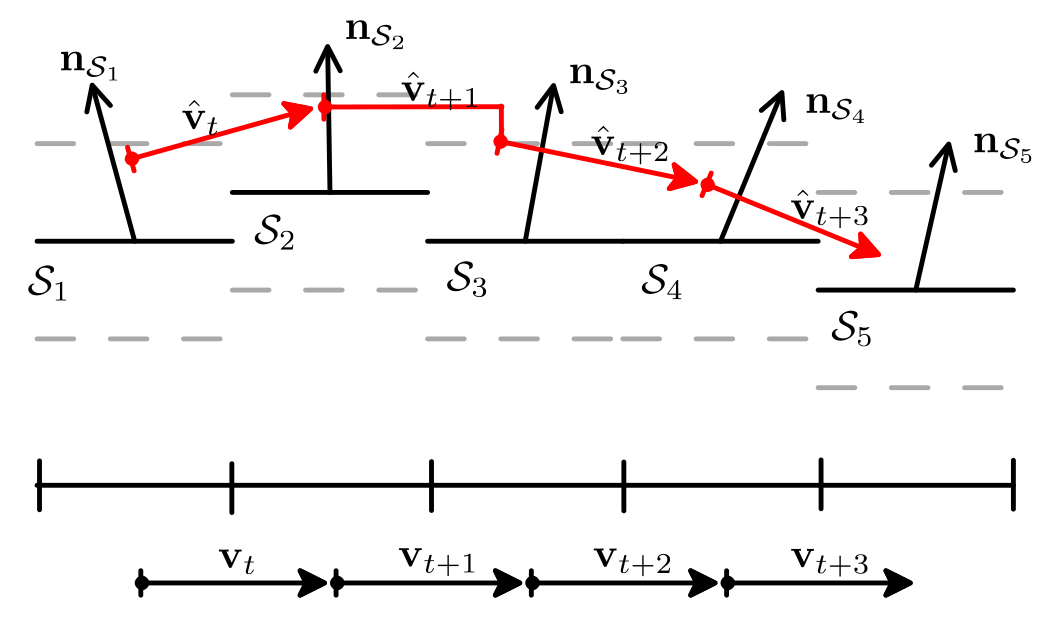
\includegraphics[width=.5\textwidth]{vector.jpg}
                \caption{Z vector\cite{article}}
                % \roundpic[xshift=0cm,yshift=0cm]{2.5cm}{6cm}{pista}
                %\caption{Pista de corrida \cite{agostini2007}}
            \end{figure}
        %}
        \end{center}
    % \end{columns}

\end{frame}

\begin{frame}[c]{\textit{Endpoint Sensor Model for MLS Maps}}
    Nesse modelo, cada raio do sensor é tratado individualmente e determinado a probabilidade de todo o scan por fatorizar todos os raios
    \newline

    \begin{center}
        \begin{figure}
            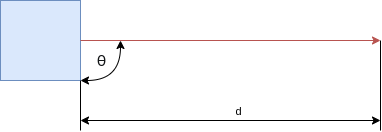
\includegraphics[width=0.5\textwidth]{sensormodel.drawio.png}
        \end{figure}
    \end{center}

    % \begin{enumerate}
    %     \item é a mistura de três distribuições(normal distribution, uniform distribution, point mass distribution);
    %     \item a probabilidade depende apenas da distância entre o raio laser e o ponto mais proximo no mapa;
    %     \item o angulo dos raios em relação ao frame do sensor são usados para definir o angulo dos obstáculos.
    % \end{enumerate}

\end{frame}

%-
%*----------- SLIDE -------------------------------------------------------------
\begin{frame}[c]{Resultados experimentais}
    \begin{figure}
        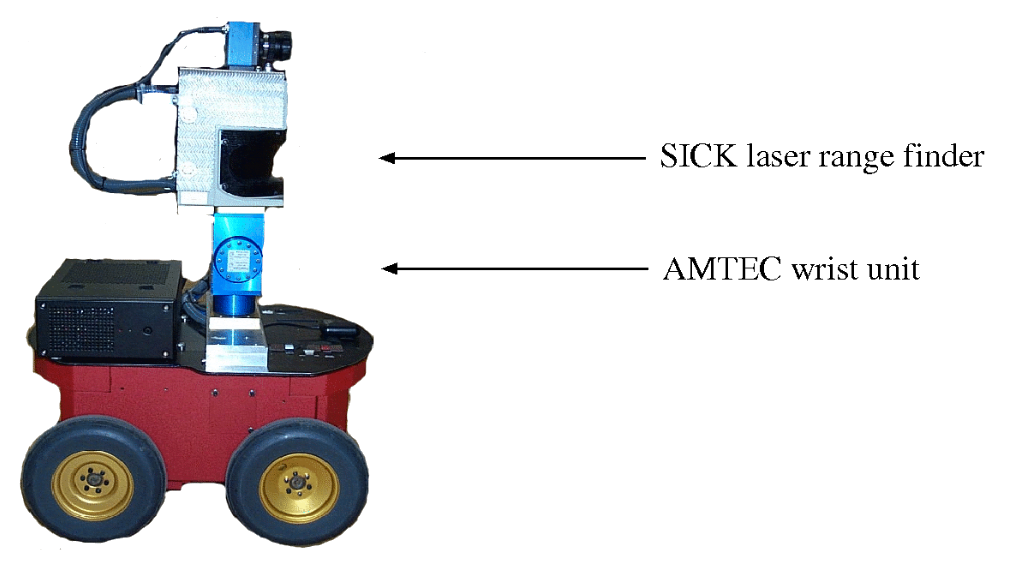
\includegraphics[width=0.7\textwidth]{robot.png}
       
        % \roundpic[xshift=0cm,yshift=0cm]{3cm}{7cm}{pista_corrida}
          
        \caption{Robô físico\cite{article}}
    \end{figure}
%*----------- notes
    \note[item]{Notes can help you to remember important information. Turn on the notes option.}
\end{frame}
%-

\begin{frame}[c]{Pode ser concluído que}
    \begin{center}
        \begin{figure}
                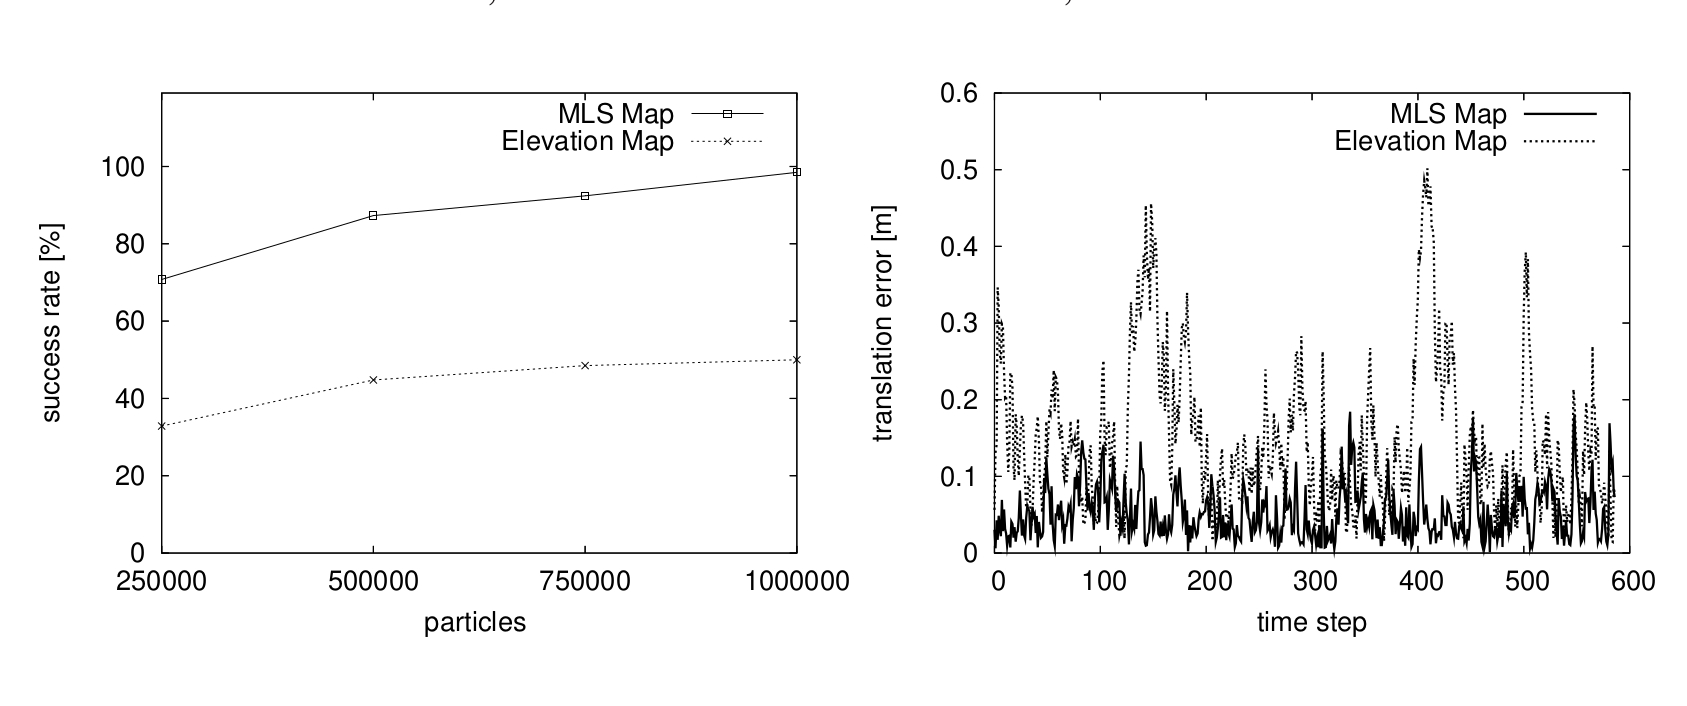
\includegraphics[width=1\textwidth]{global.jpg}
                \caption{Gráfico\cite{article}}
            \end{figure}
    \end{center}
\end{frame}

\begin{frame}[c]{Pode ser concluído que}
    \begin{center}
        \begin{figure}
                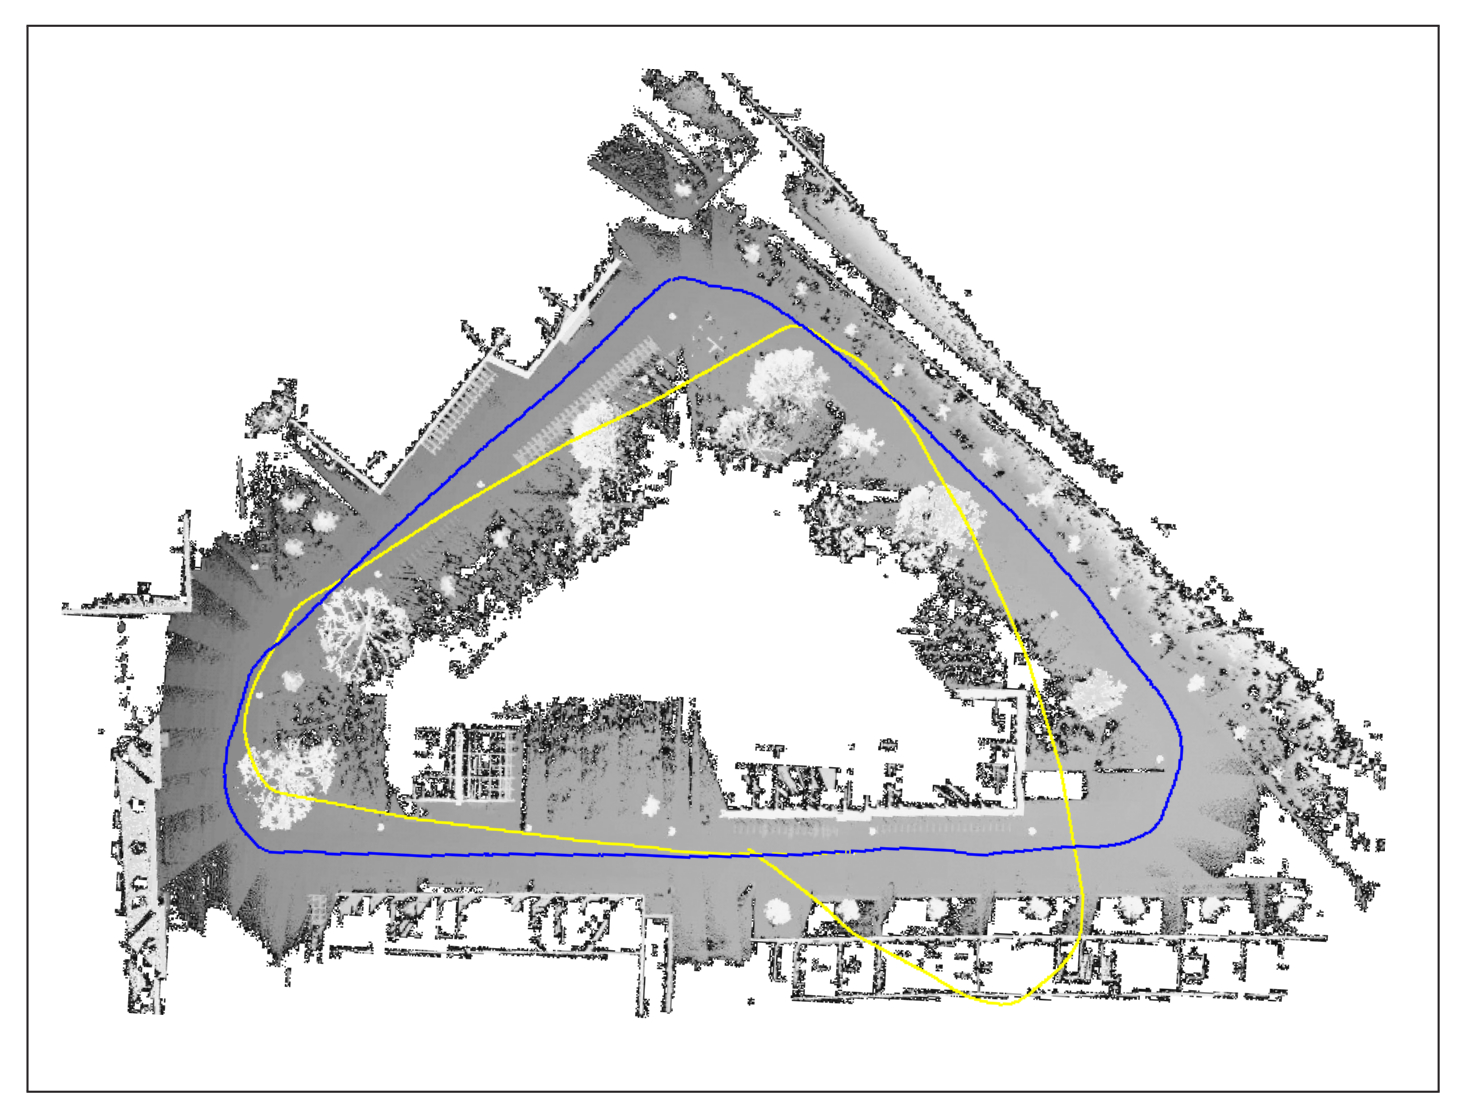
\includegraphics[width=.5\textwidth]{local.jpg}
                \caption{Resultado\cite{article}}
            \end{figure}
    \end{center}
\end{frame}